\section{Versuchsaufbau/-durchführung}
Der wesentliche Aufbau eines Sagnac Interfermoeters ist in Abildung \ref{fig:sagnac_interferometer}
dargetsellt.
\begin{figure}
\centering
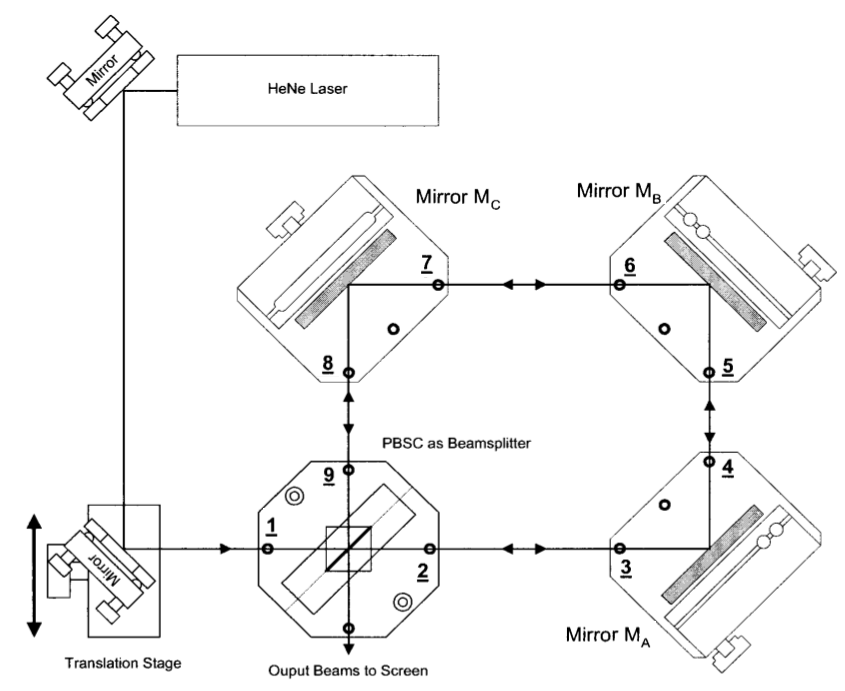
\includegraphics[width=0.7\linewidth]{./content/images/aufbau.png}
\caption{Schmeatischer Aufbau eines Sagnac Interferometers \cite{anleitung64}.}
\label{fig:sagnac_interferometer}
\end{figure}
Als Lichtquelle wird ein $\ce{HeNe}$ Laser mit einer Wellenlänge von
$\lambda\ua{vac}=\SI{632.990}$ verwendet. Der Laser wird mittels zweier Spiegel
über einen PBSC in das Interfermoeter eingeleitet. Durch dieses wird das Licht
nach durchqueren des Interferometers auch wieder ausgekoppelt.
Der Ausgangstrahl wird zur Bestimmugn des Brechungsindexes in ein weiteren
PBSC geleitet, der jedoch um $\SI{45}{\degree}$ in der Horizontalen gedreht ist.
Die Drehung des PBSC hat die selbe Auswirkung auf die Polarisation, wie ein Polarisationsfilter mit
einem Filterwinkel von $\SI{45}{\degree}$. Hierdurch wird das zunächst senkrecht
polarisierte Licht (vgl. Abb. \ref{fig:pbsc}), gedreht und ist interferenzfähig
(vgl. Gl. \eqref{}). Das von dem zweiten PBSC aufgeteiltem Licht wird
anschließend auf zwei Photodioden gerichtet.
